\chapter{An overview of \LaTeX}

In this section, a few basic tools will be presented. In following sections more advance functionality and complex tools will be showcased. \textbf{Use this guide as an example and to your advantage!}

\textsc{\color{red}Important:} this template uses Lua\LaTeX, a modern \LaTeX\ engine. You should setup your editor to use Lua\LaTeX, otherwise it will not be able to generate the document. Overleaf, for example, does not change the \LaTeX\ engine automatically, so you have to do it yourself (it is very easy!).

\textsc{\color{red}Important:} read the documentation of the pacakges that you will use! Also, read general documentation about \LaTeX! While the following guide below explains some of the most basic and cooler topics of \LaTeX, the explanations are swallow. I do not cover details nor issues that may appear and how to fix them. Some really good resources are:
\begin{itemize}
	\item \href{https://en.wikibooks.org/wiki/LaTeX}{\LaTeX's Wikibook}
	\item \href{https://www.overleaf.com/learn}{Overleaf's \LaTeX\ resources}
	\item \href{https://www.ctan.org/tex-archive/info/lshort/english/}{The not so short introduction to \LaTeX} book
	\item {\color{red} The packages' manuals!}
	\item Any searh engine.
\end{itemize}

\section{Basics of \LaTeX}

\subsection{Text styles}

The following table showcases some of the more common text styles in \LaTeX.

\begin{table}[h]
	\centering
	\begin{tabular}{lcc}
	  \toprule
	  Style & Code & Ouput \\
	  \midrule
	  Quotes & \verb|``Quotes''| & ``Quotes'' \\
	  Boldface & \verb|\textbf{Boldface}| & \textbf{Boldface} \\
	  Italics & \verb|\textit{Italics}| & \textit{Italics} \\
	  Emphasis & \verb|\emph{Emphasis}| & \emph{Emphasis} \\
	  Underline & \verb|\underline{Underline}| & \underline{Underline} \\
	  Typewriter & \verb|\texttt{Typewriter}| & \texttt{Typewriter} \\
	  Small caps & \verb|\textsc{small caps}| & \textsc{small caps} \\
	  Mathematical & \verb|$Mathematical^{\pi\cdot i}$| & $Mathematical^{\pi\cdot i}$ \\
	  \LaTeX\ Comments & \verb|% Some text| & % Some text
	  \\
	  \bottomrule
	\end{tabular}
	\caption{Text styles in \LaTeX.}
	\label{fig:textstyles}
\end{table}

\subsection{Structure of a \LaTeX\ document}

For this template, which is based in the \texttt{book} class, we have the following major sections:

\begin{enumerate}
	\item \verb|\part{}|: Parts are fully self-contained portions of information. They leave a full blank page with only the title of the part. \textbf{This is not used in this template and not recommended!}
	\item \verb|\chapter{}|: Your normal chapters, as you can see above. We are in the ``\emph{An overview of \LaTeX }'' chapter.
	\item \verb|\section{}|: Normal sections for a chapter. We are in ``\emph{Basics of \LaTeX}'' section.
	\item \verb|\subsection{}|: Subsections. We are in ``\emph{Structure of a \LaTeX\ document}'' subsection.
	\item \verb|\subsubsection{}|: Subsubsections. This level tends to be quite deep and will most likely not appear in the index unless we include \verb|\setcounter{secnumdepth}{3}|\footnote{There is also \texttt{tocdepth}, which only affects the Table of Contents.} in the preamble\footnote{The preamble is the part before \texttt{\textbackslash begin\{document\}}, basically, the setup section.}.
	\item \verb|\paragraph{}|: One step deeper. By default paragraphs are not numbered.
\end{enumerate}

You just have to write what you want between the \verb|{}| for each command, and \LaTeX\ does the rest. It typsets the titles/sections, it adds them to the table of contents and numbers them consistently!

\subsection{Structure of a \LaTeX\ paragraph}

\LaTeX\ gives us full control on how paragraphs appear in our text, but it is not obvious to know how to control such appearance.

Paragraphs can be separated by a simple empty line between themselves, with a double backslash \verb|\\| or both. However, the results these methods produce is different. Lets take a look

\begin{lstlisting}[language={[LaTeX]TeX}]
This is a test without double backslash. Take a look at how the next paragraph is indented. This is the main difference with respect to the next method shown below.

This would be the beginning of the new paragraph. There is no blank line with the previous one.
\end{lstlisting}

This is a test without double backslash. Take a look at how the next paragraph is indented. This is the main difference with respect to the next method shown below.

This would be the beginning of the new paragraph. There is no blank line with the previous one.

\begin{lstlisting}[language={[LaTeX]TeX}]
Now, lets see how the new paragraph is formated when we end this paragraph with a double backslash (\verb|\\|) and without an empty line. \\
This would be the beginning of the new paragraph. This paragraph was not indented.
\end{lstlisting}

Now, lets see how the new paragraph is formated when we end this paragraph with a double backslash (\verb|\\|) and without an empty line. \\
This would be the beginning of the new paragraph. This paragraph was not indented.

\begin{lstlisting}[language={[LaTeX]TeX}]
Now, lets see how the new paragraph is formated when we end this paragraph with a double backslash (\verb|\\|) and an empty line. \\

This would be the beginning of the new paragraph.
\end{lstlisting}

Now, lets see how the new paragraph is formated when we end this paragraph with a double backslash (\verb|\\|) and an empty line. \\

This would be the beginning of the new paragraph.

\subsection{Enumerations, bullet points and descriptions in \LaTeX}

Enumerated lists can be created with the \verb|enumerate| environment.

\begin{enumerate}
		\item First item.
		\item Second one.
	\begin{enumerate}
			\item Going deeeeper.
	\end{enumerate}
		\item Third.
\end{enumerate}

\begin{lstlisting}[language={[LaTeX]TeX}]
\begin{enumerate}
		\item First item.
		\item Second one.
	\begin{enumerate}
			\item Going deeeeper.
	\end{enumerate}
		\item Third.
\end{enumerate}
\end{lstlisting}

Bullet points or lists can be created with the \verb|itemize| environment. The structure is the same as the \verb|enumerate| environment!

\begin{itemize}
		\item First item.
		\item Second one.
	\begin{itemize}
			\item Going deeeeper.
	\end{itemize}
		\item Third.
\end{itemize}

\begin{lstlisting}[language={[LaTeX]TeX}]
\begin{itemize}
		\item First item.
		\item Second one.
	\begin{itemize}
			\item Going deeeeper.
	\end{itemize}
		\item Third.
\end{itemize}
\end{lstlisting}

Descriptions are quite nice is you need to descrive different concepts. They are created with the \verb|description| environment and the \verb|\item| entry requires the optional argument: \verb|\item[Some text]|.

\begin{description}
		\item[My favourite] First item. Lets write some more text to see the full formatting of the \verb|description| environment.
		\item[Continuation] Second one.
		\item[Finally] Third.
\end{description}

\begin{lstlisting}[language={[LaTeX]TeX}]
\begin{description}
		\item[My favourite] First item. Lets write some more text to see the full formatting of the \verb|description| environment.
		\item[Continuation] Second one.
		\item[Finally] Third.
\end{description}
\end{lstlisting}

\subsection{Mathematical notation}

\LaTeX\ provides several way to include symbols and write mathematical formulas. The most basic way is to include mathematical notation or symbols into the text. This is known as \emph{inline} and can be done with \verb|$...$|. Whatever is between the \$ symbols, is typeset in mathematical notation. This is an example: $2 = \frac{4}{2}$. This is produced using \verb|$2 = \frac{4}{2}$|.

Another method is to write mathematical formulas in \emph{display} mode, which is separated from the text. This can be done by wrapping the text in \verb|\[...\]|. \textbf{This is not recommended} as the next method is better. Here is an example:

\[
	2 = \frac{4}{2}
\]

Normally, the best way is to use mathematical environments. This environments will provide more functionality and generally number the equations and allows them to be labelled. Here are a few examples:

\begin{equation} \label{eq:simpleeq}
	2 = \frac{4}{2}
\end{equation}

The equation above, \cref{eq:simpleeq}, is produced by writing:

\begin{lstlisting}[language={[LaTeX]TeX}]
\begin{equation} \label{eq:simpleeq}
	2 = \frac{4}{2}
\end{equation}
\end{lstlisting}

Lets showcase more environments that help us write beautiful formulas! The \verb|\begin{array}| environment helps us write vertically aligned formulas!

\begin{equation} \label{eq:abaqus-exponential-decay}
f(t) = \left\{
	\begin{array}{lcc}
		A_0 + A\cdot e^{-\dfrac{t - t_0}{t_d}} & for & t \geq t_0 \\
		A_0 & for & t < t_0
	\end{array}
	\right.
\end{equation}

\begin{lstlisting}[language={[LaTeX]TeX}]
\begin{equation} \label{eq:abaqus-exponential-decay}
	f(t) = \left\{
	\begin{array}{lcc}
		A_0 + A\cdot e^{-\dfrac{t - t_0}{t_d}} & for & t \geq t_0 \\
		A_0 & for & t < t_0
	\end{array}
	\right.
\end{equation}
\end{lstlisting}


The \verb|\begin{aling}| environment may be easier to use, but it has a few quirks. Read the documentation\footnote{\url{http://tug.ctan.org/info/short-math-guide/short-math-guide.pdf}} for more information.

\begin{align}
	a_{11}& =b_{11}&
	a_{12}& =b_{12}\\
	a_{21}& =b_{21}&
	a_{22}& =b_{22}+c_{22}
\end{align}

\begin{lstlisting}[language={[LaTeX]TeX}]
\begin{align}
	a_{11}& =b_{11}&
	a_{12}& =b_{12}\\
	a_{21}& =b_{21}&
	a_{22}& =b_{22}+c_{22}
\end{align}
\end{lstlisting}

The \verb|\begin{subequations}| allows us to have several formulas numbered into the same reference. As shown in \cref{eq:symmetry-bc}, with the first entry being \cref{eq:x-symmetry-bc}.

\begin{subequations} \label{eq:symmetry-bc}
	\begin{equation} \label{eq:x-symmetry-bc}
		\text{\texttt{XSYMM}} \equiv U1 = UR2 = UR3 = 0
	\end{equation}
	\begin{equation}
		\text{\texttt{ZSYMM}} \equiv U3 = UR1 = UR2 = 0
	\end{equation}
\end{subequations}

\begin{lstlisting}[language={[LaTeX]TeX}]
\begin{subequations} \label{eq:symmetry-bc}
	\begin{equation} \label{eq:x-symmetry-bc}
		\text{\texttt{XSYMM}} \equiv U1 = UR2 = UR3 = 0
	\end{equation}
	\begin{equation}
		\text{\texttt{ZSYMM}} \equiv U3 = UR1 = UR2 = 0
	\end{equation}
\end{subequations}
\end{lstlisting}

\subsection{References}

One of the strongest points of \LaTeX\ is its wonderful and powerful referencing system. We can reference whatever we want by putting on a ``tag'' with the command \verb|\label{xxx}|. Wherever the \verb|\label| is, it will refer to it. You can see some examples above where we refered to a few equations by their labels, which are inside the \verb|\begin{equation}| environment. This way, \LaTeX\ knows automatically what type of thing they are referring.

The different types of references are shown in \cref{tab:reference-systems}.

\begin{table}[h]
	\centering
	\begin{tabular}{lcc}
	  \toprule
	  Package & Command & Result \\
	  \midrule
	  \LaTeX & \verb|\ref{eq:simpleeq}| & \ref{eq:simpleeq} \\
	  & \verb|\pageref{eq:simpleeq}| & \pageref{eq:simpleeq} \\
	  \cmidrule{2-3}
	  \texttt{hyperref} & \verb|\autoref{eq:simpleeq}| & \autoref{eq:simpleeq} \\
			  & \verb|\autoref{fig:textstyles}| & \autoref{fig:textstyles} \\
			  & \verb|\autopageref{eq:simpleeq}| & \autopageref{eq:simpleeq} \\
	  \cmidrule{2-3}
	  \texttt{cleveref} & \verb|\cref{eq:simpleeq}| & \cref{eq:simpleeq} \\
			  & \verb|\Cref{eq:simpleeq}| & \Cref{eq:simpleeq} \\
	  & \verb|\cpageref{eq:simpleeq}| & \cpageref{eq:simpleeq} \\
			  & \verb|\cref{eq:simpleeq,eq:symmetry-bc}| & \cref{eq:simpleeq,eq:symmetry-bc} \\
			  & \verb|\crefrange{eq:simpleeq}| & \multirow{2}{*}{\crefrange{eq:simpleeq}{eq:symmetry-bc}}\\
	  & \verb|{eq:symmetry-bc}| & \\
	  \bottomrule
	\end{tabular}
	\caption[Different reference mechanisms.]{Different reference mechanisms. \textbf{The author recommends \texttt{cleveref}!}. It is included in this template.}
	\label{tab:reference-systems}
\end{table}

The style of references created by \texttt{cleveref} can be changed to use a full word by setting the \texttt{noabbrev} option in the \texttt{report.tex} file. The relevant line is \verb|\usepackage[nameinlink]{cleveref}|.

\subsection{Bibliography}

Bibliography management is another strong point of \LaTeX! We just need to add bibliographic entries to the bibliography database, which for this template it is the \texttt{main.bib} file. Here is what such an entry can look like:

\begin{lstlisting}[language={[LaTeX]TeX}]
@book{lovecraft2016el,
	author = {Lovecraft, H. P.},
	title = {El clérigo malvado y otros relatos},
	publisher = {Alianza Editorial},
	year = {2016},
	address = {Madrid},
	isbn = {9788491042105}
}
\end{lstlisting}

In order to cite the entry we just have to use \verb|\cite{}| with the entry's identifier, like so \verb|\cite{lovecraft2016el}| \cite{lovecraft2016el}. We can also have multiple cites in the same command, \cite{lovecraft2016el,norton_creep} (\verb|\cite{lovecraft2016el,norton_creep}|). It is that simple! They get automatically printed in the bibliography section.

\textsc{\color{red}Important:} this template uses \texttt{biblatex} as the management system, which is a powerful, flexible and modern tool. Therefore, you will need to run the \texttt{biber} command to build the bibliography after the first compilation of your document; then you will have to recompile the document after \texttt{biber} has run. Most editors do this by default.

You can also use third-party tools like Zotero\footnote{\url{https://www.zotero.org/}} to manage your \verb|.bib| database. Most bibliography management tools are capable of dealing with \verb|.bib| entries!

\subsection{Tables, images and floating environments}

Probably, the part of \LaTeX\ that causes the most confusion among new users, are the so called \emph{floating envrionments}. \textbf{Tables, images, algorithms, etc are floating envrionments}. This means that \textbf{\LaTeX\ can position them where it sees fit, not where they are written by the user.} In reality, \LaTeX\ is trying to optimise your document's layout and leave as little empty space as possible.

Sooo... How do we solve \LaTeX\ moving our floating environments? Here are a few solutions:

\begin{itemize}
	\item We don't solve it. \LaTeX\ referencing tools allow us to easily point the reader to the table, image, etc. Therefore, it is not that problematic that the \emph{floats} may not be where we put them!
	\item We can ask \LaTeX\ to try to place the image where it appears in our document. This is done with the \emph{``here''} \verb|[h]| placement modifier. More on placement modifiers later. \textbf{This is not a definitive solution.} This will just tell \LaTeX\ to try hard to do what we are asking. There is the \verb|[h!]| modifier, which is even stronger.
	\item \textbf{A really good solution is to use} \verb|\FloatBarrier|. It comes from the \verb|placeins| package, included in this template. \verb|\FloatBarrier| forces \LaTeX\ to put all floating environment that have already appeared before the position where \verb|\FloatBarrier| appears. This is very useful to force \LaTeX\ to put all floats before another section that may not be related to the topic of those floats. Here is an example:

\begin{lstlisting}[language={[LaTeX]TeX}]
\section{Some topic}

\begin{figure}
	XXX
\end{figure}

\begin{table}
	XXX
\end{table}

\FloatBarrier % All previous floats will appear before this point.

\section{Some unrelated topic}
XXX
\end{lstlisting}
	\item We can use the placement modifier \verb|[H]| to force the float to appear \emph{HERE}. This is provided by the \verb|float| package. However, \textbf{this solution is not recommended!} It can lead to some wierd and nasty document layouts!
\end{itemize}

Now, how do we actually include figures, tables, etc? They all follow the same structure, here are some examples:

\begin{description}
		\item[Figures] are declared in the \verb|figure| environment (\emph{\textsc{shock!}}). You can see the image rendered in \cref{fig:monoblock-overview-mesh}.

\begin{lstlisting}[language={[LaTeX]TeX}]
\begin{figure}
	\centering % Center image horizontally
	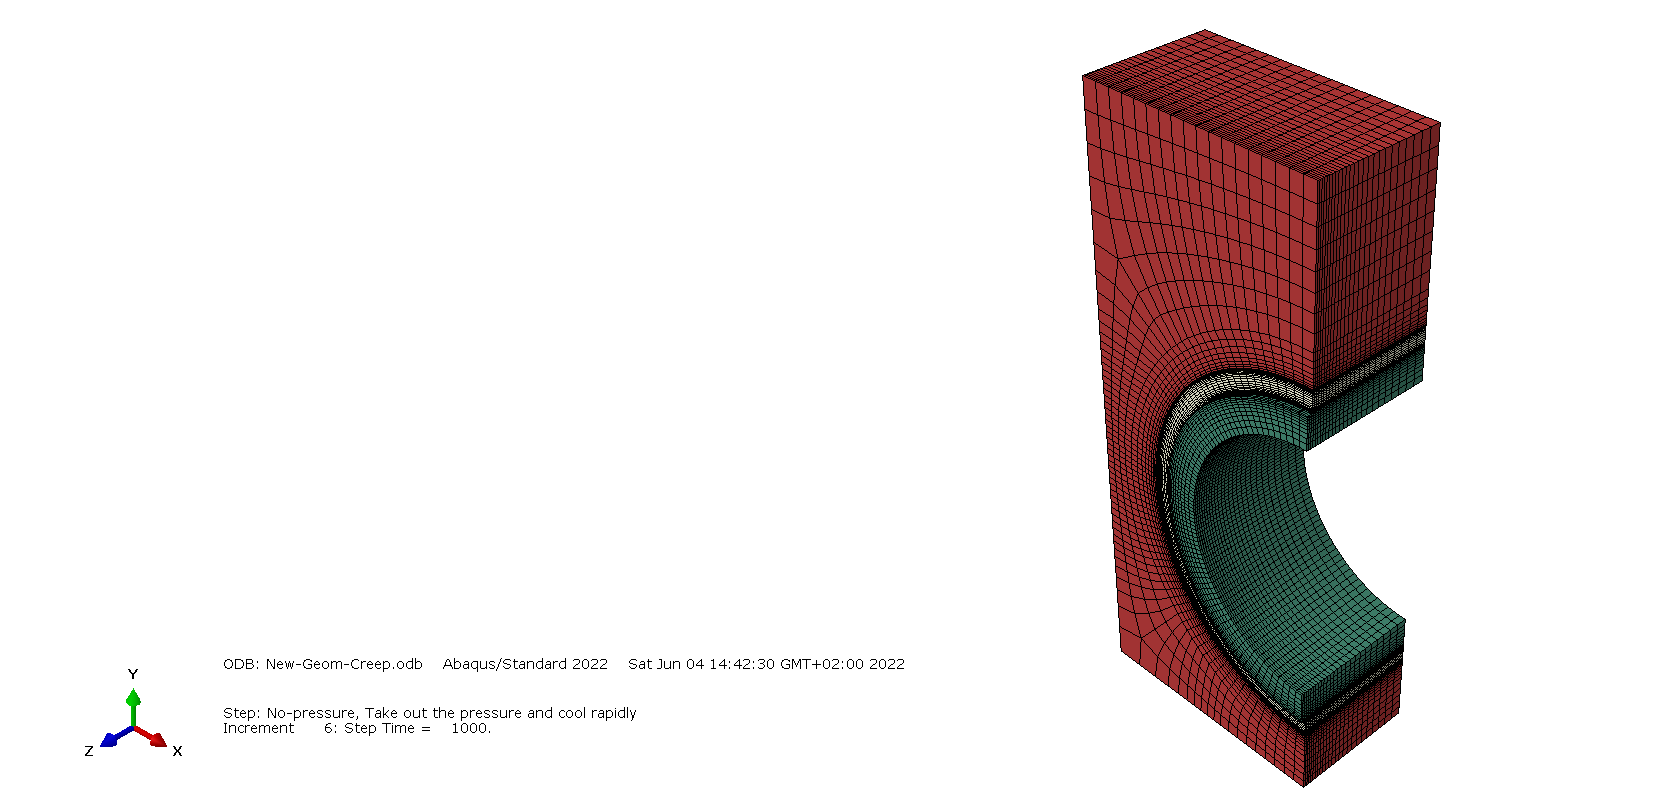
\includegraphics[keepaspectratio, trim = 1050 12 150 30, clip, width=0.5\linewidth, height=0.3\textheight]{Images/monoblock-material-overview-mesh.png}
	\caption[Overview of \glsentryname{FEM} mesh used for the final analysis.]{Overview of \glsxtrshort{FEM} mesh used for the final analysis.}
	\label{fig:monoblock-overview-mesh}
\end{figure}
\end{lstlisting}
	The key here is \verb|\includegraphics|, it is what loads the graphics and allows us to set its properties. The above example is rather complex, most times you do not need these many options. Nonetheless, here is what they do:
	\begin{description}
			\item[\texttt{keepaspectratio}] Keeps the size ratio of the image. Very useful if you set \verb|height| and \verb|width| at the same time. \verb|\includegraphics| will use the most restrictive length to size the image.
			\item[\texttt{trim}] It allows us to trim/cut the image. It cuts X amount of pixels from the \texttt{left, bottom, right, top}. This is useful if your image is too large and you only care about a small portion of it.
			\item[\texttt{clip}] Only show the trimmed image.
			\item[\texttt{width} and \texttt{height}] Sets the maximum size with respect to the width and height. We use \verb|\linewidth| and \verb|\textheight| to limit the size of the image in the page by using the page's natural lengths.
	\end{description}

	Then we have \verb|\caption|, which is what adds the text to the image. We use \verb|\caption[]| here, to modify the text that will appear in the ``List of Figures'', as I do not want my acronym \texttt{FEM} to be linked there, and therefore I use \verb|\glsentryname| to control that. But more about acronyms and glossaries in \cref{sec:glossaries}
	Finally, we have \verb|\label{}| is is what allows us to give an identifier to our image so that we can reference it.
\end{description}

\begin{figure}[h]
	\centering % Center image horizontally
	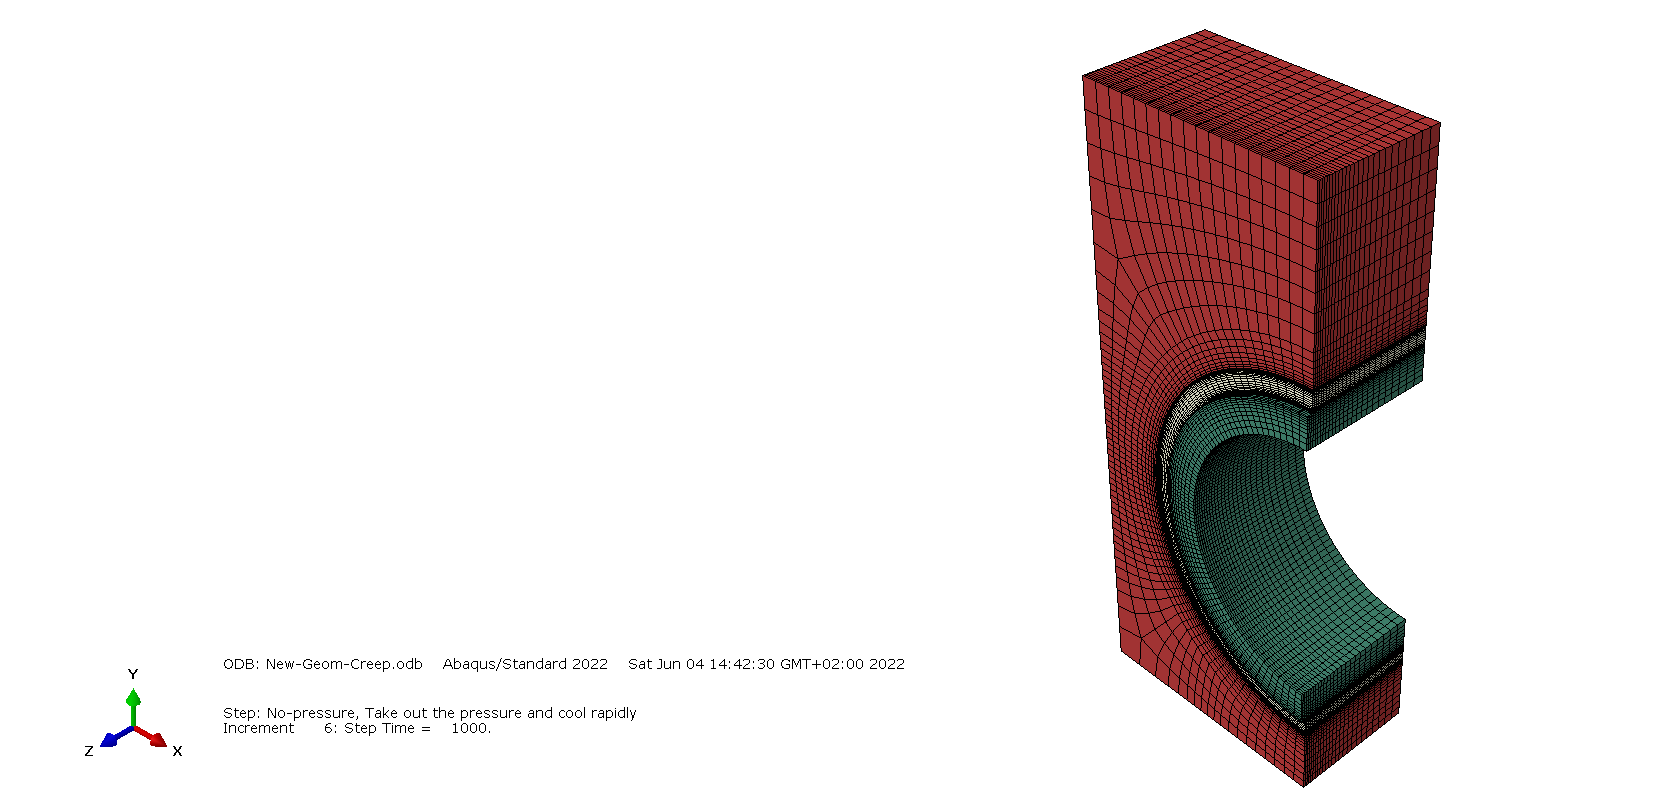
\includegraphics[keepaspectratio, trim = 1050 12 150 30, clip, width=0.5\linewidth, height=0.3\textheight]{Images/monoblock-material-overview-mesh.png}
	\caption[Overview of \glsentryname{FEM} mesh used for the final analysis.]{Overview of \glsxtrshort{FEM} mesh used for the final analysis.}
	\label{fig:monoblock-overview-mesh}
\end{figure}

\begin{description}
	\item[Tables] are fairly easy to do once we get used to their nature. It uses the \verb|table| floating environment with another environment that allows us to type tabulated data. A basic example is given below and shown in \cref{tab:example-table}.
\begin{lstlisting}[language={[LaTeX]TeX}]
\begin{table}
	\centering % To center the table
	\begin{tabular}{lcr}
	  \toprule
	  Heading 1 & Heading 2 & Heading 3 \\
	  \midrule
	  Left aligned & Center aligned & Right aligned \\
	  \cmidrule{2-3} % Example of a defined size rule
	  Some info & Some info & Some info \\
	  \bottomrule
	\end{tabular}
	\caption{Example of a table.}
	\label{tab:example-table}
\end{table}
\end{lstlisting}
	\textsc{\color{red}Important:} the \texttt{\&} symbol is used as a column separator in all alignment environments! Go back to the mathematical environments and see if you can see its use there.

	The column alingment options for the tabular environment can be \texttt{l, c, r, m{}} or \texttt{p{}} among others. They refer to left, center, right alignment and the \texttt{m{}} and \texttt{p{}} refer to a limited size column whose vertical alignment is either centered or natural. You could use them as \verb|m{0.3\linewidth}| for example. If you want to aling the text horizontally with \texttt{m} or \texttt{p} you would write \verb|>{\centering\arraybackslash}m{0.3\linewidth}|. You can change the \verb|\centering| for a \verb|\raggedright| for a right aligned column. But this is getting too advance!
	One final bit of knowledge about very long tables and dynamicly sized columns. This template includes the package \texttt{xltabular}, which includes the well-known \verb|tabularx| environment and merges it with the \verb|longtable| environment (for tables that can span more than one page) generating its own \verb|xltabular| envrionment. Please read the documentation of the \texttt{tabularx}, \verb|longtable| and \verb|xltabular| packages if you need to build complex tables!

	There are also two packages \verb|multicolumn| and \verb|multirow| that allows the content of a cell to span several columns/rows. These packages are included in this template. Take a look at their documentation.

	Also, \textbf{there are online tools to help you generate \LaTeX\ tables from Excel sheets}. One such example (which I am not very familiar with nor endorse) is \href{https://tableconvert.com/excel-to-latex}{Tableconvert}.

	Finally, if you have \texttt{.csv} files or similar and you want to print them in your \LaTeX\ document, you can see \cref{sec:pgfplotstable}, which shows how \cref{tab:automatic-reading-csv} was automatically generated using \verb|pgfplotstable|.
\end{description}

\begin{table}[h]
	\centering % To center the table
	\begin{tabular}{lcr}
	  \toprule
	  Heading 1 & Heading 2 & Heading 3 \\
	  \midrule
	  Left aligned & Center aligned & Right aligned \\
	  \cmidrule{2-3} % Example of a controled rule
	  Some info & Some info & Some info \\
	  \bottomrule
	\end{tabular}
	\caption{Example of a table.}
	\label{tab:example-table}
\end{table}

See \cref{sec:subcaption} for an example on how to have several labeled pictures, tables, etc in a single environment.

\FloatBarrier

\section{Glossaries}\label{sec:glossaries}

Creating glossaries in \LaTeX\ is surprisingly easy. However, it does require a bit of understanding.

For this template, the entries for the glossaries and acronyms (which are just a different type of glossary) are loaded from the \texttt{glossaries.tex} and \texttt{acronyms.tex} files. This is just to keep things organised. So, lets define some entries for our glossary and acronym list.

For glossary entries we use the \verb|\newglossaryentry{}{...}| command. Here is an example:

\begin{lstlisting}[language={[LaTeX]TeX}]
\newglossaryentry{identifier}
{
	name={name}, % Mandatory, what gets printed
	description={description of the entry}, % Mandatory, description that appears in the glossary index
	plural={plural-name}, % Optional, in case the plural is more complex
	sort={alphanumeric entry}, % Optional, how should the entry be sorted
	symbol={\ensuremath{associated symbol}}, % Optional, prints the symbol of the entry with \glssymbol{identifier}
}
\end{lstlisting}

For acronyms, we could use the code above, but there is a simpler and more direct way of doing it with \verb|\newabbreviation[]{}{}{}|. Here is how it works:

\begin{lstlisting}[language={[LaTeX]TeX}]
\newabbreviation{Identifier}{ACRONYM}{Description Of Acronym}
\end{lstlisting}

\verb|\newabbreviation[]| supports a long set of options. For example, the \verb|[longplural={...}]| option allows us to write the plural form in case it is more refined. There are many other options. The abbreviation functionality is provided by the \verb|glossaries-extra| package.

Once your own personal entries have been created, you can use them with the following commands.

\begin{table}[h]
	\centering
	\begin{tabular}{lcc}
	  \toprule
	  Type & Command & Result \\
	  \midrule
	  Glossary & \verb|\gls{test}| & \gls{test} \\
		   & \verb|\Gls{test}| & \Gls{test} \\
		   & \verb|\glspl{test}| & \glspl{test} \\
		   & \verb|\Glspl{test}| & \Glspl{test} \\
		   & \verb|\glsentryname{test}| & \glsentryname{test} \\
		   & \multicolumn{2}{l}{$\uparrow$ this does not produce a link} \\
	  \cmidrule{2-3}
	  Acronyms & \verb|\glsxtrshort{FEM}| & \glsxtrshort{FEM} \\
		   & \verb|\glsxtrshortpl{FEM}| & \glsxtrshortpl{FEM} \\
		   & \verb|\glsxtrlong{FEM}| & \glsxtrlong{FEM} \\
		   & \verb|\glsxtrfull{FEM}| & \glsxtrfull{FEM} \\
		   & \verb|\glsentryname{FEM}| & \glsentryname{FEM} \\
	   & \verb|\gls{FEM}| & \gls{FEM} \\
	  What? & \verb|\gls{FEM}| & \gls{FEM} \\
	  \bottomrule
	\end{tabular}
	\caption{Glossary and acronym types.}
	\label{tab:glossaries}
\end{table}

\FloatBarrier

Wait, what happened in the second \verb|\gls{FEM}| entry in the acronym section? Why did it produce a different result (\verb|\glsxtrshort{FEM}|) when compared to the first one (\verb|\glsxtrfull{FEM}|)?

Simple. This template uses the \verb|\setabbreviationstyle[acronym]{long-short}| style. The first time an acronym is used, it will show the full form. After that, the short form is used. All of this automatically! Isn't this magical? If you would like to show always the short form, you can delete that line from the \texttt{report.tex} or use \verb|\setabbreviationstyle[acronym]{short-nolong}| (or any other style that you like!).

\textsc{\color{red}Important:} in order to show the list of glossaries and acronyms in their table of contents, you will have to run \verb|makeglossaires|. Some editors will do that automatically for you, as they will detect you have a glossary in your document.

\section{Automatic loading and formatting of code}

The package included in this template, \verb|listings|, allows us to format code into our document. You have already seen it in action multiple times! All the code examples in this introduction have been generated by \verb|listings|.

The package has two ways of formatting code in our document. The first method, \textbf{which is not ideal,} is to explicitly write/copy the code into the \verb|lstlisting| environment. Here is an example:

\begin{lstlisting}[language=Ada, caption={Hello world in Ada}, label={lst:hello-world-ada}]
with Ada.Text_IO; use Ada.Text_IO;

procedure Hello_World is
begin
    Put_Line ("Hello World");
end Hello_World;
\end{lstlisting}

\lstnewenvironment{TeXlstlisting}{\lstset{language=[LaTeX]TeX}}{}

\begin{TeXlstlisting}
\begin{lstlisting}[language=Ada, caption={Hello world in Ada}, label={lst:hello-world-ada}]
with Ada.Text_IO; use Ada.Text_IO;

procedure Hello_World is
begin
    Put_Line ("Hello World");
end Hello_World;
\end{lstlisting}
\end{TeXlstlisting}

A slightly better way is to read the file that has already been written and typeset it directly. This can be achieved using \verb|\lstinputlisting|. Here is an example:

\lstinputlisting
[
language={[77]Fortran},
firstline=154,
caption={Abaqus' \texttt{CREEP} subroutine example for several materials.},
label={lst:subroutine-creep-materials}
]
{Data/Cu_CuCrZr_creep_secondary.for}

\begin{TeXlstlisting}
\lstinputlisting
[
language={[77]Fortran},
firstline=154,
caption={Abaqus' \texttt{CREEP} subroutine example for several materials.},
label={lst:subroutine-creep-materials}
]
{Data/Cu_CuCrZr_creep_secondary.for}
\end{TeXlstlisting}

If you are going to be printing code of the same programming language constantly, it is easier to set the language to be used globally. This can be done with \verb|\lstset{language=[LaTeX]TeX}| for example.

The colours, style, etc of the listings are defined in the \verb|loaded-thesis.sty| file, which is the main body of this template. You can modify it to your liking!

\section{Creating beautiful plots in 2D and 3D}

Oh... This is an interesting and impresive part. But I must warn new \LaTeX\ users: doing plots in \LaTeX\ with \verb|pgfplots| is not a trivial thing and takes a bit of practice! Read its documentation, as it is an incredibly capable package!

\subsection{Plots with formulas}

We can create simple plots by directly writing the formula. The first part of this example is the configuration of the \verb|axis|, which is the section that controls the axis, style, etc of our plot. Once it is configured, we can start adding plots using the different \verb|\addplot| command styles. Lets see an example:

\begin{figure}[h]
	\centering
	\begin{tikzpicture} % PGFplots uses TikZ to draw the plots
		\begin{axis}[ % Define the actual plot parameters
			title={Title of the plot},
			width=0.95\textwidth,
			height=0.4\textheight,
			xlabel={\glsxtrshort{HRP} time [\unit{\hour}]},
			ylabel={Temperature [\unit{\celsius}]},
			grid=major, % How fine we want the grid
			enlarge x limits=false, % By default, the axis are enlarged 
			axis x discontinuity=crunch, % Our domain does not start at zero, add discontinuity
			xmin=19, % Start value for X
			xtickmin=20, % First tick for X
			ymin=0,
			ymax=600,
			ytick distance=50, % Interval for which the labels are printed
			legend pos=north east, % Were the legend should go
			legend cell align=left,
			ylabel near ticks,
			]

			% Start adding lines!
			\addplot [
			thick, % Thickness of the line
			red, % Colour of the line
			domain=20.5:35.75 % For what domain of X the expression should be computed
			] % And now, the actual formula
			{580*exp(-(x-20.5)/(27050/60/60))};
			% IMPORTANT, notice the trailing semicolon (;)!
			% Add line to legend
			\addlegendentry{Exponential decrease}

			\addplot [
			thick,
			blue,
			domain=35.75:36.15
			]
			{-112*x+4080};
			\addlegendentry{Linear decrease}
		\end{axis}
	\end{tikzpicture}
	\caption{Caption of our plot}
	\label{fig:temperature-time-transient}
\end{figure}

\begin{TeXlstlisting}
\begin{figure}[h]
	\centering
	\begin{tikzpicture} % PGFplots uses TikZ to draw the plots
		\begin{axis}[ % Define the actual plot parameters
			title={Title of the plot},
			width=0.95\textwidth,
			height=0.4\textheight,
			xlabel={\glsxtrshort{HRP} time [\unit{\hour}]},
			ylabel={Temperature [\unit{\celsius}]},
			grid=major, % How fine we want the grid
			enlarge x limits=false, % By default, the axis are enlarged 
			axis x discontinuity=crunch, % Our domain does not start at zero, add discontinuity
			xmin=19, % Start value for X
			xtickmin=20, % First tick for X
			ymin=0,
			ymax=600,
			ytick distance=50, % Interval for which the labels are printed
			legend pos=north east, % Were the legend should go
			legend cell align=left,
			ylabel near ticks,
			]

			% Start adding lines!
			\addplot [
			thick, % Thickness of the line
			red, % Colour of the line
			domain=20.5:35.75 % For what domain of X the expression should be computed
			] % And now, the actual formula
			{580*exp(-(x-20.5)/(27050/60/60))};
			% IMPORTANT, notice the trailing semicolon (;)!
			% Add line to legend
			\addlegendentry{Exponential decrease}

			\addplot [
			thick,
			blue,
			domain=35.75:36.15
			]
			{-112*x+4080};
			\addlegendentry{Linear decrease}
		\end{axis}
	\end{tikzpicture}
	\caption{Caption of our plot}
	\label{fig:temperature-time-transient}
\end{figure}
\end{TeXlstlisting}

We can also do 3D plots! The plot in \cref{fig:3d-plot} uses glossaries in its entries, and parametised values at the top. \textbf{However, this parametrisation of values is not recommended,} as it forces \verb|pgfplots| to use a slower engine.

\begin{figure}[h]
	% Define values for plots
	% Variables
	\newcommand\Nexp{4.8}
	\newcommand\Mexp{0.0}
	\newcommand\Acoeff{38.8}
	\newcommand\SIGMAMIN{5}
	\newcommand\SIGMAMAX{150}
	% Min Temp 100C
	\newcommand\TEMPMIN{75}
	% Max Temp 600C
	\newcommand\TEMPMAX{600}
	% Self-diffusion energy
	\newcommand\Q{197000}
	\centering
	\begin{tikzpicture}
		\begin{axis}[
			title={$\dot{\epsilon}_{cr} = \Acoeff \cdot \gls{stressdevia}^{\Nexp} \cdot e^{\left(-\frac{\Q}{\gls{gasconstant}\cdot \gls{temperature}_{abs}}\right)}$},
			width=0.8\textwidth,
			xlabel={\gls{stressdevia} [\unit{\mega\pascal}]},
			ylabel={\gls{temperature} [\unit{\celsius}]},
			ytick distance=100,
			xtick distance=50,
			zlabel={\gls{creepstrainrate}\ [\unit{\per\second}]},
			zmode=log, % Logarithmic axis!
			grid=major,
			colormap/viridis, % Select colour
			% view={0}{90}, % View from the top
			]

			\addplot3 [
			thick,
			surf,
			domain=\SIGMAMIN:\SIGMAMAX,
			y domain=\TEMPMIN:\TEMPMAX,
			samples=50,
			samples y=50,
			]
			% Formula as a function of X and Y
			{\Acoeff*x^\Nexp*exp(-\Q/(8.314*(y+273.15)))};
		\end{axis}
	\end{tikzpicture}
	\caption{Yup, 3D plots are that easy! And this one is parametised}
	\label{fig:3d-plot}
\end{figure}

\begin{TeXlstlisting}
\begin{figure}[h]
	% Define values for plots
	% Variables
	\newcommand\Nexp{4.8}
	\newcommand\Mexp{0.0}
	\newcommand\Acoeff{38.8}
	\newcommand\SIGMAMIN{5}
	\newcommand\SIGMAMAX{150}
	% Min Temp 100C
	\newcommand\TEMPMIN{75}
	% Max Temp 600C
	\newcommand\TEMPMAX{600}
	% Self-diffusion energy
	\newcommand\Q{197000}
	\centering
	\begin{tikzpicture}
		\begin{axis}[
			title={$\dot{\epsilon}_{cr} = \Acoeff \cdot \gls{stressdevia}^{\Nexp} \cdot e^{\left(-\frac{\Q}{\gls{gasconstant}\cdot \gls{temperature}_{abs}}\right)}$},
			width=0.8\textwidth,
			xlabel={\gls{stressdevia} [\unit{\mega\pascal}]},
			ylabel={\gls{temperature} [\unit{\celsius}]},
			ytick distance=100,
			xtick distance=50,
			zlabel={\gls{creepstrainrate}\ [\unit{\per\second}]},
			zmode=log, % Logarithmic axis!
			grid=major,
			colormap/viridis, % Select colour
			% view={0}{90}, % View from the top
			]

			\addplot3 [
			thick,
			surf,
			domain=\SIGMAMIN:\SIGMAMAX,
			y domain=\TEMPMIN:\TEMPMAX,
			samples=50,
			samples y=50,
			]
			% Formula as a function of X and Y
			{\Acoeff*x^\Nexp*exp(-\Q/(8.314*(y+273.15)))};
		\end{axis}
	\end{tikzpicture}
	\caption{Yup, 3D plots are that easy! And this one is parametised}
	\label{fig:3d-plot}
\end{figure}
\end{TeXlstlisting}

\subsection{Plots with data from files}

\texttt{PGFplots} can easily read, plot and even transform data from files. The data needs to be provided in a somewhat tabulated manner. Your typical \texttt{.cvs} or \texttt{.dat} files will do fine. This is done with the \verb|\addplot [] table [] {}| command. The first set of options refers to the plotting style, the second one, to the reading and interpretation of data; finally, the argument points to the file.

\texttt{PGFplots} can modify the data that it reads. This allows a lot of really nice tricks; like reading \texttt{X} and \texttt{Y} coordinate data and using them to generate \texttt{Z} values with a formula for a 3D plot!

\begin{figure}[h]
	\centering
	\begin{tikzpicture}
		\pgfplotsset{set layers}
		\begin{axis}[
			title={Mises stress evolution.},
			width=0.9\textwidth,
			height=0.375\textheight,
			xlabel={Time [\unit{\second}]},
			ylabel={\gls{stressdevia} [\unit{\mega\pascal}]},
			enlargelimits=false,
			grid=major,
			ymax=120,
			% Carefully position the legend
			legend style={
				at={(axis cs:12500, 80)}, anchor=south west
			}
			]

			% Add a legend title
			\addlegendimage{empty legend}
			\addlegendentry[text width=0.2\textwidth, align=center]{\textbf{Stress}}
			\addplot [
			thick,
			blue
			] table
			% Now we setup the columns that are read and the type of separator
			[col sep=semicolon, x index=0, y index = 3, header=false]
			% And the file with the data
			{Data/Creep-Cu-external-PEEQ-S-TEMP.csv};
			\addlegendentry{Cu-e}

			\addplot [
			thick,
			color=green!60!black
			] table
			[col sep=semicolon, x index=0, y index = 3, header=false]
			{Data/Creep-Cu-internal-PEEQ-S-TEMP.csv};
			\addlegendentry{Cu-c}
		\end{axis}
	\end{tikzpicture}
	\caption{Stress history.}
	\label{fig:stress-evolution}
\end{figure}

\begin{TeXlstlisting}
\begin{figure}[h]
	\centering
	\begin{tikzpicture}
		\pgfplotsset{set layers}
		\begin{axis}[
			title={Mises stress evolution.},
			width=0.9\textwidth,
			height=0.375\textheight,
			xlabel={Time [\unit{\second}]},
			ylabel={\gls{stressdevia} [\unit{\mega\pascal}]},
			enlargelimits=false,
			grid=major,
			ymax=120,
			% Carefully position the legend
			legend style={
				at={(axis cs:12500, 80)}, anchor=south west
			}
			]

			% Add a legend title
			\addlegendimage{empty legend}
			\addlegendentry[text width=0.2\textwidth, align=center]{\textbf{Stress}}
			\addplot [
			thick,
			blue
			] table
			% Now we setup the columns that are read and the type of separator
			[col sep=semicolon, x index=0, y index = 3, header=false]
			% And the file with the data
			{Data/Creep-Cu-external-PEEQ-S-TEMP.csv};
			\addlegendentry{Cu-e}
			\addplot [
			thick,
			color=green!60!black
			] table
			[col sep=semicolon, x index=0, y index = 3, header=false]
			{Data/Creep-Cu-internal-PEEQ-S-TEMP.csv};
			\addlegendentry{Cu-c}
		\end{axis}
	\end{tikzpicture}
	\caption{Stress history.}
	\label{fig:stress-evolution}
\end{figure}
\end{TeXlstlisting}

\subsection{Grouped plots}

Finally, lets showcase how grouped plots work. In the following example, we use the \verb|groupplot| environment instead of the \verb|axis| one. Then using the \verb|\nextgroupplot[]| command, we can configure the next plot that will be shown.

On top of showcasing how groupplots work, the following example also showcases how to write text on top of the plot and how to colour the background. This process is automated for all plots by defining the anotations and background as a global setting that then we add to each plot.

This example may seem overwhelming, but there is a lot of repetition, so do not fear it and read the comments in the code!

%% Define some constants that will be used in all plots, so that we don't have to repeat ourselves!
% Color and background definition
\definecolor{W}{RGB}{161, 51, 51}
\definecolor{Cu}{RGB}{211, 211, 190}
\definecolor{CuCrZr}{RGB}{45, 91, 76}

% Define the background colour and the text that will be used in all plots
% The distance set in the coordinates are relative axis.
% This means that it is relative to the size of the plot, which allows it to be reused in all plots!
\newcommand{\ColourMaterialBackground}{
	\begin{pgfonlayer}{axis background}
		% Tungsten
		\fill[shade, top color=W!20, bottom color=W!5]
		(rel axis cs:0,0)--(rel axis cs:0.762,0)--
		(rel axis cs:0.762,1)--(rel axis cs:0,1)--cycle;
		% Copper
		\fill[shade, top color=Cu!20, bottom color=Cu!5]
		(rel axis cs:0.762,0)--(rel axis cs:0.857,0)--
		(rel axis cs:0.857,1)--(rel axis cs:0.762,1)--cycle;
		% CuCrZr
		\fill[shade, top color=CuCrZr!20, bottom color=CuCrZr!5]
		(rel axis cs:0.857,0)--(rel axis cs:1,0)--
		(rel axis cs:1,1)--(rel axis cs:0.857,1)--cycle;
	\end{pgfonlayer}
	% Add text to the plot
	\node[anchor = south] at (axis cs: 4, 200) {\small W};
	\node[anchor = south] at (axis cs: 8.5, 200) {\small Cu};
	\node[anchor = north, text centered, text width = 15pt] at (axis cs: 9.75, 200) {\small Cu Cr Zr};
}

\begin{figure}[h]
	\centering
	\begin{tikzpicture}
		% Create group plot
		\begin{groupplot}[
			% Begin configuring how the plots are grouped
			group style = {
				group size = 2 by 2,
				horizontal sep = 10pt, % Horizontal distance
				ylabels at = edge left, % Where the y label should appear
				y descriptions at = edge left, % Same
				x descriptions at = edge bottom, % Only show abcissa at the bottom
				vertical sep = 10pt % Vertical disctance
			},
			% Here the common axis settings for all plots are given
			title style={text width=0.4\textwidth, align=center,},
			width=0.52\textwidth,
			grid=major,
			xlabel={Depth [mm]},
			enlarge x limits=false,
			ylabel near ticks
			]

			% First plot
			\nextgroupplot[
			% Title of first plot
			title={Stress distribution, edge line (green).},
			% Y label for the first plot
			ylabel={\gls{stressdevia} [\unit{\mega\pascal}]},
			% Set min and max values to make it share boundaries with the next plot
			ymin=0,
			ymax=500,
			% Position legend
			legend pos=north west,
			legend cell align=left,
			% VERY IMPORTANT. We need the layers to paint the backgound
			set layers
			]

			% Add plots as you would normally do
			\addplot [
			thick,
			blue
			] table
			[col sep=semicolon, x index=0, y index = 1, header=false]
			{Data/Mises-no-creep-ext-ext2-internal.csv};
			\addlegendentry{Without creep}
			\addplot [
			thick,
			red
			] table
			[col sep=semicolon, x index=0, y index = 1, header=false]
			{Data/Mises-creep-ext-ext2-internal.csv};
			\addlegendentry{With creep}
			% Add the background and annotations
			\ColourMaterialBackground

			% Next plot!
			\nextgroupplot[
			% Set its title
			title={Stress distribution, center line (purple).},
			% Set the same min and max as before!
			ymin=0,
			ymax=500,
			% Once again, we need the layers!
			set layers
			]

			\addplot [
			thick,
			blue
			] table
			[col sep=semicolon, x index=0, y index = 5, header=false]
			{Data/Mises-no-creep-ext-ext2-internal.csv};
			\addplot [
			thick,
			red
			] table
			[col sep=semicolon, x index=0, y index = 5, header=false]
			{Data/Mises-creep-ext-ext2-internal.csv};
			% Add background and annotations
			\ColourMaterialBackground

			% Third plot
			\nextgroupplot[
			ylabel={$\sigma_{Hoop}$ [\unit{\mega\pascal}]},
			ymax=575,
			ymin=-400,
			% Once again, we need to activate layer manipulation
			set layers
			]

			\addplot [
			thick,
			blue
			] table
			[col sep=semicolon, x index=0, y index = 3, header=false]
			{Data/Hoop-no-creep-ext-ext2-internal.csv};
			\addplot [
			thick,
			red
			] table[col sep=semicolon, x index=0, y index = 3, header=false]
			{Data/Hoop-creep-ext-ext2-internal.csv};
			% Add background and annotations
			\ColourMaterialBackground

			% Fourth and final plot!
			\nextgroupplot[
			ymax=575,
			ymin=-400,
			% Activate layers
			set layers
			]

			\addplot [
			thick,
			blue
			] table
			[col sep=semicolon, x index=0, y index = 5, header=false]
			{Data/Hoop-no-creep-ext-ext2-internal.csv};
			\addplot [
			thick,
			red
			] table
			[col sep=semicolon, x index=0, y index = 5, header=false]
			{Data/Hoop-creep-ext-ext2-internal.csv};
			% Add background and annotations
			\ColourMaterialBackground
		\end{groupplot}
	\end{tikzpicture}
	\caption[Mises and hoop stress comparison between the model without creep and the one with creep in \glsentryname{Cu-OFHC}.]{Mises and hoop stress comparison between the model without creep and the one with creep in \glsxtrshort{Cu-OFHC}.}
	\label{fig:plot-stress-creep-no-creep}
\end{figure}

\begin{TeXlstlisting}
%% Define some constants that will be used in all plots, so that we don't have to repeat ourselves!
% Color and background definition
\definecolor{W}{RGB}{161, 51, 51}
\definecolor{Cu}{RGB}{211, 211, 190}
\definecolor{CuCrZr}{RGB}{45, 91, 76}

% Define the background colour and the text that will be used in all plots
% The distance set in the coordinates are relative axis.
% This means that it is relative to the size of the plot, which allows it to be reused in all plots!
\newcommand{\ColourMaterialBackground}{
	\begin{pgfonlayer}{axis background}
		% Tungsten
		\fill[shade, top color=W!20, bottom color=W!5]
		(rel axis cs:0,0)--(rel axis cs:0.762,0)--
		(rel axis cs:0.762,1)--(rel axis cs:0,1)--cycle;
		% Copper
		\fill[shade, top color=Cu!20, bottom color=Cu!5]
		(rel axis cs:0.762,0)--(rel axis cs:0.857,0)--
		(rel axis cs:0.857,1)--(rel axis cs:0.762,1)--cycle;
		% CuCrZr
		\fill[shade, top color=CuCrZr!20, bottom color=CuCrZr!5]
		(rel axis cs:0.857,0)--(rel axis cs:1,0)--
		(rel axis cs:1,1)--(rel axis cs:0.857,1)--cycle;
	\end{pgfonlayer}
	% Add text to the plot
	\node[anchor = south] at (axis cs: 4, 200) {\small W};
	\node[anchor = south] at (axis cs: 8.5, 200) {\small Cu};
	\node[anchor = north, text centered, text width = 15pt] at (axis cs: 9.75, 200) {\small Cu Cr Zr};
}

\begin{figure}[h]
	\centering
	\begin{tikzpicture}
		% Create group plot
		\begin{groupplot}[
			% Begin configuring how the plots are grouped
			group style = {
				group size = 2 by 2,
				horizontal sep = 10pt, % Horizontal distance
				ylabels at = edge left, % Where the y label should appear
				y descriptions at = edge left, % Same
				x descriptions at = edge bottom, % Only show abcissa at the bottom
				vertical sep = 10pt % Vertical disctance
			},
			% Here the common axis settings for all plots are given
			title style={text width=0.4\textwidth, align=center,},
			width=0.52\textwidth,
			grid=major,
			xlabel={Depth [mm]},
			enlarge x limits=false,
			ylabel near ticks
			]

			% First plot
			\nextgroupplot[
			% Title of first plot
			title={Stress distribution, edge line (green).},
			% Y label for the first plot
			ylabel={\gls{stressdevia} [\unit{\mega\pascal}]},
			% Set min and max values to make it share boundaries with the next plot
			ymin=0,
			ymax=500,
			% Position legend
			legend pos=north west,
			legend cell align=left,
			% VERY IMPORTANT. We need the layers to paint the backgound
			set layers
			]

			% Add plots as you would normally do
			\addplot [
			thick,
			blue
			] table
			[col sep=semicolon, x index=0, y index = 1, header=false]
			{Data/Mises-no-creep-ext-ext2-internal.csv};
			\addlegendentry{Without creep}
			\addplot [
			thick,
			red
			] table
			[col sep=semicolon, x index=0, y index = 1, header=false]
			{Data/Mises-creep-ext-ext2-internal.csv};
			\addlegendentry{With creep}
			% Add the background and annotations
			\ColourMaterialBackground

			% Next plot!
			\nextgroupplot[
			% Set its title
			title={Stress distribution, center line (purple).},
			% Set the same min and max as before!
			ymin=0,
			ymax=500,
			% Once again, we need the layers!
			set layers
			]

			\addplot [
			thick,
			blue
			] table
			[col sep=semicolon, x index=0, y index = 5, header=false]
			{Data/Mises-no-creep-ext-ext2-internal.csv};
			\addplot [
			thick,
			red
			] table
			[col sep=semicolon, x index=0, y index = 5, header=false]
			{Data/Mises-creep-ext-ext2-internal.csv};
			% Add background and annotations
			\ColourMaterialBackground

			% Third plot
			\nextgroupplot[
			ylabel={$\sigma_{Hoop}$ [\unit{\mega\pascal}]},
			ymax=575,
			ymin=-400,
			% Once again, we need to activate layer manipulation
			set layers
			]

			\addplot [
			thick,
			blue
			] table
			[col sep=semicolon, x index=0, y index = 3, header=false]
			{Data/Hoop-no-creep-ext-ext2-internal.csv};
			\addplot [
			thick,
			red
			] table[col sep=semicolon, x index=0, y index = 3, header=false]
			{Data/Hoop-creep-ext-ext2-internal.csv};
			% Add background and annotations
			\ColourMaterialBackground

			% Fourth and final plot!
			\nextgroupplot[
			ymax=575,
			ymin=-400,
			% Activate layers
			set layers
			]

			\addplot [
			thick,
			blue
			] table
			[col sep=semicolon, x index=0, y index = 5, header=false]
			{Data/Hoop-no-creep-ext-ext2-internal.csv};
			\addplot [
			thick,
			red
			] table
			[col sep=semicolon, x index=0, y index = 5, header=false]
			{Data/Hoop-creep-ext-ext2-internal.csv};
			% Add background and annotations
			\ColourMaterialBackground
		\end{groupplot}
	\end{tikzpicture}
	\caption[Mises and hoop stress comparison between the model without creep and the one with creep in \glsentryname{Cu-OFHC}.]{Mises and hoop stress comparison between the model without creep and the one with creep in \glsxtrshort{Cu-OFHC}.}
	\label{fig:plot-stress-creep-no-creep}
\end{figure}
\end{TeXlstlisting}

\section{Automatic formatting of table data} \label{sec:pgfplotstable}

The following table, \cref{tab:automatic-reading-csv}, is formatted using the following general setup for \verb|pgfplotstable|. The following \LaTeX-\verb|pgfplotstable| is only needed once, and it applies to ``all'' the automatically loaded table.

\begin{lstlisting}[language={[LaTeX]TeX}]
% Configure the general setting of pgfplotstable
\pgfplotstableset{
	every odd row/.style={
		before row={\rowcolor{gray!20}}
	},
	every head row/.style={
		before row=\toprule,
		after row=\midrule,
		% Don't print the row name or the row index!
		output empty row
	},
	every last row/.style={
		after row=\bottomrule
	},
	header=false,
	format=file,
	col sep=tab,
	search path={Data},
	font={\small}
}
\end{lstlisting}

And then the actual loading of the table. The following code setups the header (names, columns, etc) and then loads the data.
\begin{lstlisting}[language={[LaTeX]TeX}]
\begin{table}
	\newcommand{\prop}{Expansion}
	\newcommand{\propunit}{[\unit{\milli\meter\per\celsius\per\milli\meter}]}
	\centering
	\pgfplotstabletypeset[
	every head row/.append style={
		before row={
			\toprule
			\multicolumn{2}{c}{\glsentryname{Cu-OFHC}} \\
			\midrule
			\multirow{2}{\widthof{\propunit}}{\centering \prop\ \propunit} & \multirow{2}{\widthof{Temperature}}{\centering Temperature [\unit{\celsius}]} \\
			\\
		},
	},
	]{ITER Cu You-harden for WPDIV phase II_\prop_f_T.txt}
	\caption{Automatically formatted table using \texttt{pgfplotstable}.}
	\label{tab:automatic-reading-csv}
\end{table}
\end{lstlisting}

Whats even cooler is that \verb|pgfplotstable| uses the package \verb|siunitx| to format the values as it is included in this template!

% Configure the general setting of pgfplotstable
\pgfplotstableset{
	every odd row/.style={
		before row={\rowcolor{gray!20}}
	},
	every head row/.style={
		before row=\toprule,
		after row=\midrule,
		% Don't print the row name or the row index!
		output empty row
	},
	every last row/.style={
		after row=\bottomrule
	},
	header=false,
	format=file,
	col sep=tab,
	search path={Data},
	font={\small}
}

\begin{table}[h]
	\newcommand{\prop}{Expansion}

\newcommand{\propunit}{[\unit{\milli\meter\per\celsius\per\milli\meter}]}
	\centering
	\pgfplotstabletypeset[
	every head row/.append style={
		before row={
			\toprule
			\multicolumn{2}{c}{\glsentryname{Cu-OFHC}} \\
			\midrule
			\multirow{2}{\widthof{\propunit}}{\centering \prop\ \propunit} & \multirow{2}{\widthof{Temperature}}{\centering Temperature [\unit{\celsius}]} \\
			\\
		},
	},
	]{ITER Cu You-harden for WPDIV phase II_\prop_f_T.txt}
	\caption{Automatically formatted table using \texttt{pgfplotstable}.}
	\label{tab:automatic-reading-csv}
\end{table}

\section{Writing algorithms}

Using the \verb|algorithm2e| package, we can format beautiful algorithms. Here is an example from my thesis. The algorithm is \cref{alg:fib-deletion} and the geometrical explanation is shown in \cref{fig:fib-geometry}. Also, notice that the algorithm is on a left page (even number) and the picture is on the right (odd number page). In \cref{sec:extra-bits} I explain how to achive this result. As always, \textsc{read the documentation of the package!}

\begin{genericfloat} % I added this extra bit, because otherwise leftfullpage fails to work!
	\begin{leftfullpage}
		\begin{algorithm}[H]
			\KwData{\texttt{USDFLD} input parameters, including field and time $(0 < t \leq 1)$ data}
			\KwResult{Set the field and state to deleted if required}
			\tcc{See \autoref{fig:fib-geometry} for a geometrical description of the algorithm}
			\BlankLine
			\tcc{Define geometrical parameters}
			\Begin{
				\tcc{User defined parameters}
				$r_i := r_i$\tcc*[r]{Inner radius}
				$r_o := r_o$\tcc*[r]{Outer radius}
				$\vec{C} := \{C_x, C_y, C_z\}$\tcc*[r]{Cylinder center}
				$\vec{V} := \{V_x, V_y, V_z\}$\tcc*[r]{Unit displacement vector}
				\BlankLine
				\tcc{Gauss element position, input from Abaqus}
				$\vec{G} := \{G_x, G_y, G_z\}$\;
				\BlankLine
				\tcc{Computed location of cylinder at step time \gls{timestep}}
				$\vec{C}^* := \vec{C} + \vec{V} \cdot \gls{timestep}$\;
			}
			\BlankLine
			\tcc*[l]{Compute intersection of Gauss elements and geometry}
			\Begin{
				\tcc{Element distance from the center}
				$\vec{D} := \vec{G} - \vec{C}^*$\;
				\tcc{Project distance over to the displacement vector}
				$m := \vec{D} \cdot \vec{V}$\;
				\tcc{Check if the element is behind the advancing front}
				\If{$m \leq 0.0$}{
					\tcc{Distance from $\vec{G}$ to the cylinder axis}
					$d := \| \vec{D} - m\cdot \vec{V} \|$\;
					\tcc{Check if the Gauss element is between the radii}
					\If{$d \leq r_o \wedge d \geq r_i$}{
						Field$_G$ := 0\tcc*[r]{Disable element}
						State$_G$ := 0\tcc*[r]{Set state to deleted}
					}
				}
			}
			\caption[Full logic used for the \glsentryname{FIB}--\glsentryname{DIC} element deletion operation.]{Full logic used for the \glsxtrshort{FIB}--\glsxtrshort{DIC} element deletion operation. The algorithm assumes the cylinder axis is the same as the displacement vector.}
			\label{alg:fib-deletion}
		\end{algorithm}
	\end{leftfullpage}
\end{genericfloat}

\begin{figure}
	\begin{fullpage}
		\centering
		\def\svgwidth{\linewidth}
		\import{Data}{fib-vectors.pdf_tex}
		\caption[Geometry description for element deletion in a \glsentryname{FIB}--\glsentryname{DIC} case.]{Geometry description for element deletion in a \glsxtrshort{FIB}--\glsxtrshort{DIC} case. In this example, $G_2$ would be considered outside of the geometry as its distance to the axis is smaller than $r_i$. $G_1$ is within $r_i$ and $r_o$ and behind $\vec{C}^*$ as $m \leq 0.0$, so it would have been deleted. We simplify the problem by assuming the cylinder's axis is the same as the displacement vector.}
		\label{fig:fib-geometry}
	\end{fullpage}
\end{figure}

\begin{TeXlstlisting}
\begin{genericfloat} % I added this extra bit, because otherwise leftfullpage fails to work!
	\begin{leftfullpage}
		\begin{algorithm}[H]
			\KwData{\texttt{USDFLD} input parameters, including field and time $(0 < t \leq 1)$ data}
			\KwResult{Set the field and state to deleted if required}
			\tcc{See \autoref{fig:fib-geometry} for a geometrical description of the algorithm}
			\BlankLine
			\tcc{Define geometrical parameters}
			\Begin{
				\tcc{User defined parameters}
				$r_i := r_i$\tcc*[r]{Inner radius}
				$r_o := r_o$\tcc*[r]{Outer radius}
				$\vec{C} := \{C_x, C_y, C_z\}$\tcc*[r]{Cylinder center}
				$\vec{V} := \{V_x, V_y, V_z\}$\tcc*[r]{Unit displacement vector}
				\BlankLine
				\tcc{Gauss element position, input from Abaqus}
				$\vec{G} := \{G_x, G_y, G_z\}$\;
				\BlankLine
				\tcc{Computed location of cylinder at step time \gls{timestep}}
				$\vec{C}^* := \vec{C} + \vec{V} \cdot \gls{timestep}$\;
			}
			\BlankLine
			\tcc*[l]{Compute intersection of Gauss elements and geometry}
			\Begin{
				\tcc{Element distance from the center}
				$\vec{D} := \vec{G} - \vec{C}^*$\;
				\tcc{Project distance over to the displacement vector}
				$m := \vec{D} \cdot \vec{V}$\;
				\tcc{Check if the element is behind the advancing front}
				\If{$m \leq 0.0$}{
					\tcc{Distance from $\vec{G}$ to the cylinder axis}
					$d := \| \vec{D} - m\cdot \vec{V} \|$\;
					\tcc{Check if the Gauss element is between the radii}
					\If{$d \leq r_o \wedge d \geq r_i$}{
						Field$_G$ := 0\tcc*[r]{Disable element}
						State$_G$ := 0\tcc*[r]{Set state to deleted}
					}
				}
			}
			\caption[Full logic used for the \glsentryname{FIB}--\glsentryname{DIC} element deletion operation.]{Full logic used for the \glsxtrshort{FIB}--\glsxtrshort{DIC} element deletion operation. The algorithm assumes the cylinder axis is the same as the displacement vector.}
			\label{alg:fib-deletion}
		\end{algorithm}
	\end{leftfullpage}
\end{genericfloat}
\end{TeXlstlisting}

\FloatBarrier

\section{Some extra bits of knowledge} \label{sec:extra-bits}

\subsection{Subcaptions, multiple floats together} \label{sec:subcaption}

The \verb|subcaption| package, included in this template, allows us to display and label several floating entries in the same environment. Here is an example for figures:

\begin{figure}[h]
	\centering
	\begin{subfigure}{0.3\textwidth}
		\centering
		\includegraphics[width=\hsize]{example-image-a}
		\caption{Bird A}
		\label{fig:bird-a}
	\end{subfigure}
	\hfill % Fill the horizontal space
	\begin{subfigure}{0.3\textwidth}
		\centering
		\includegraphics[width=\hsize]{example-image-b}
		\caption{Bird B}
		\label{fig:bird-a}
	\end{subfigure}
	\hfill
	\begin{subfigure}{0.3\textwidth}
		\centering
		\includegraphics[width=\hsize]{example-image-c}
		\caption{Bird C}
		\label{fig:bird-a}
	\end{subfigure}
	\caption{Birds. Taken from \href{https://tex.stackexchange.com/questions/343605/latex-code-for-subcaption-of-image}{this forum post}.}
	\label{fig:birds-1}
\end{figure}

\begin{TeXlstlisting}
\begin{figure}[h]
	\centering
	\begin{subfigure}{0.3\textwidth}
		\centering
		\includegraphics[width=\hsize]{example-image-a}
		\caption{Bird A}
		\label{fig:bird-a}
	\end{subfigure}
	\hfill % Fill the horizontal space
	\begin{subfigure}{0.3\textwidth}
		\centering
		\includegraphics[width=\hsize]{example-image-b}
		\caption{Bird B}
		\label{fig:bird-a}
	\end{subfigure}
	\hfill
	\begin{subfigure}{0.3\textwidth}
		\centering
		\includegraphics[width=\hsize]{example-image-c}
		\caption{Bird C}
		\label{fig:bird-a}
	\end{subfigure}
	\caption{Birds. Taken from \href{https://tex.stackexchange.com/questions/343605/latex-code-for-subcaption-of-image}{this forum post}.}
	\label{fig:birds-1}
\end{figure}
\end{TeXlstlisting}

\subsection{How do I change the colour of the citations/references?}

This template by default uses colours for links so that you, the user, can distinguish them. However, colours may not be wanted. The colour setting are present in \texttt{report.tex}, under \verb|\hypersetup{}|. The defaults for this template are shown below.

If you do not want colours set \verb|colorlinks| to \verb|false|. If you also dislike the boxes that appear in the PDF view, set \verb|hidelinks| to true (in this template, just uncomment the line!).

\begin{TeXlstlisting}
\hypersetup{
	colorlinks = true, % Colour links. Set to false to let the text be black
	citecolor = red,
	urlcolor = blue,
	linkcolor = red,
%	hidelinks = true, % Uncomment to hide all link indications, such as boxes
} % Change this options to your liking
\end{TeXlstlisting}

\subsection{How do I prevent \LaTeX\ from splitting a word, number, etc?}

\LaTeX\ will automatically break some words or numbers in order to have a nice layout of the paragraph. However, sometime we don't want that. This can be solved with \verb|\mbox{XXX}|. This, however, may generate unexpecte behaviour! For example: \mbox{\texttt{XXXXXXXXXXXXXXXXXXXXXXXXXXXXXXXXXXXXXXXXXXXXXXXXXXXXXXXXXXXXXXXXXXXXXXXXXXXXXXXXXX}}.

\subsection[Can I put two figures, tables, etc; side to side?]{Can I put two figures, tables, etc; side to side? One on the left page and another thing on the right page.}

Yes! With the package \verb|dpfloat|, included in the template. \textbf{However, it can generate a lot of errors} if \LaTeX\ cannot put enough text around the floating environments\footnote{The error tends to be \texttt{Output loop---100 consecutive dead cycles.}}. The easiest solution is to write a bit more text or place the floats more deeply into your text.

Here is a demonstration of an example from my thesis. Inside your \texttt{figure, table, etc}, use the \verb|leftfullpage| environment around the contents to place something in the left page. Then in the next float environment, which should be written directly next to the previous one, use the \verb|fullpage| environment. Here is an example with \cref{fig:boundary-conditions} and \cref{tab:fem-steps}.

\begin{lstlisting}[language={[LaTeX]TeX}]
\begin{figure}
	\begin{leftfullpage} % Place in the left page
	\centering
	\def\svgwidth{0.6\linewidth}
	\import{Data}{BCs.pdf_tex} % Import LaTeX graphics generated by Inkscape!
	\caption[\glsentryname{FEM} boundary conditions.]{Boundary conditions applied on the monoblock.}
	\label{fig:boundary-conditions}
	\end{leftfullpage}
\end{figure}
\end{lstlisting}

\begin{figure}
	\begin{leftfullpage} % Place in the left page
	\centering
	\def\svgwidth{0.6\linewidth}
	\import{Data}{BCs.pdf_tex} % Import LaTeX graphics generated by Inkscape!
	\caption[\glsentryname{FEM} boundary conditions.]{Boundary conditions applied on the monoblock.}
	\label{fig:boundary-conditions}
	\end{leftfullpage}
\end{figure}

\begin{lstlisting}[language={[LaTeX]TeX}]
\begin{table}
	\begin{fullpage} % Put it in a right page
			\centering
			\footnotesize
			\begin{tabularx}{\linewidth}{>{\raggedright\arraybackslash}X >{\centering\arraybackslash}X >{\centering\arraybackslash}X >{\centering\arraybackslash}X >{\centering\arraybackslash}X >{\centering\arraybackslash}X}
			  \toprule
			  & Pressure increase & Exponential drop of temperature & Rapid drop of temperature & Cutting of cooling pipe & Cutting of the part \\
			  \cmidrule(r){2-4} \cmidrule(l){5-6}
			  Duration & \qty{10}{\second} & \qty{55000}{\second} & \qty{1000}{\second} & \qty{1}{\second} & \qty{1}{\second} \\
			  \midrule
			  Temperature  & \qty{580}{\celsius} & \qtyrange[range-units=single]{580}{76}{\celsius} & \qtyrange[range-units=single]{76}{20}{\celsius} & \qty{20}{\celsius} & \qty{20}{\celsius} \\
			  \midrule
			  .
			  .
			  .
			  \bottomrule
			\end{tabularx}
			\caption{Simulated steps and their boundary conditions.}
			\label{tab:fem-steps}
	\end{fullpage}
\end{table}
\end{lstlisting}

\begin{table}
	\begin{fullpage} % Put it in a right page
			\centering
			\footnotesize
			\begin{tabularx}{\linewidth}{>{\raggedright\arraybackslash}X >{\centering\arraybackslash}X >{\centering\arraybackslash}X >{\centering\arraybackslash}X >{\centering\arraybackslash}X >{\centering\arraybackslash}X}
			  \toprule
			  & Pressure increase & Exponential drop of temperature & Rapid drop of temperature & Cutting of cooling pipe & Cutting of the part \\
			  \cmidrule(r){2-4} \cmidrule(l){5-6}
			  Duration & \qty{10}{\second} & \qty{55000}{\second} & \qty{1000}{\second} & \qty{1}{\second} & \qty{1}{\second} \\
			  \midrule
			  Temperature  & \qty{580}{\celsius} & \qtyrange[range-units=single]{580}{76}{\celsius} & \qtyrange[range-units=single]{76}{20}{\celsius} & \qty{20}{\celsius} & \qty{20}{\celsius} \\
			  \midrule
			  \glsxtrshort{HRP} pressure & \qtyrange[range-units=single]{0}{10}{\mega\pascal} & \qty{10}{\mega\pascal} & \qtyrange[range-units=single]{10}{0}{\mega\pascal} & --- & --- \\
			  \midrule
			  Tie constrains & \checkmark & \checkmark & \checkmark & \checkmark &  \checkmark \\
			  \midrule
			  X Symmetry plane & \checkmark & \checkmark & \checkmark & \checkmark &  \checkmark \\
			  Z Symmetry plane & \checkmark & \checkmark & \checkmark & \checkmark &  \checkmark \\
			  Y = 0 \mbox{bottom plane} & \checkmark & \checkmark & \checkmark & \checkmark & ---  \\
			  \midrule
			  Planar \glsxtrshort{BC} & \checkmark & \checkmark & \checkmark & ---  & --- \\
			  \midrule
			  Vertical fix of top and bottom center point & --- & --- & --- & --- & \checkmark \\
			  \bottomrule
			\end{tabularx}
			\caption{Simulated steps and their boundary conditions.}
			\label{tab:fem-steps}
		\end{fullpage}
\end{table}

\subsection{How can I edit graphics in \LaTeX?}

In the \verb|figure| explanation at the beginning of the chapter I show how you can clip the graphics in \LaTeX. However, if you would like to add text, arrows and similar things to your graphics, \textbf{the best way is to use \href{https://inkscape.org/}{Inkscape}}. It is a vector/image manipulation program that can ouput files to be loaded and typsetted by \LaTeX! You can see \cref{fig:boundary-conditions}, which is generated with Inkscape (file named \texttt{BCs.svg} in the \texttt{Data} directory). \href{https://tex.stackexchange.com/questions/151232/exporting-from-inkscape-to-latex-via-tikz}{This forum post} explains how to do it.
% Emacs setup

%%% Local Variables:
%%% mode: latex
%%% coding: utf-8
%%% TeX-engine: luatex
%%% TeX-master: "../report"
%%% End:
